% This is part of Un soupçon de mathématique sans être agressif pour autant
% Copyright (c) 2014
%   Laurent Claessens
% See the file fdl-1.3.txt for copying conditions.

%+++++++++++++++++++++++++++++++++++++++++++++++++++++++++++++++++++++++++++++++++++++++++++++++++++++++++++++++++++++++++++ 
\section{Origami}
%+++++++++++++++++++++++++++++++++++++++++++++++++++++++++++++++++++++++++++++++++++++++++++++++++++++++++++++++++++++++++++

La feuille distribuée pour la découverte du théorème d'Haga.

% THÉORÈME DE HAGA POUR L'AP
\begin{feuilleExo}{Théorème de Haga}

%\begin{wrapfigure}{r}{10.cm}
    \begin{center}
\includegraphics[width=10cm]{Haga}
    \end{center}
%\end{wrapfigure}

\paragraph{Un peu de Pythagore}


Nous avons appelé \( a\) la longueur du segment \( [AC]\). Pourquoi \( BC=1-a\) ? Quelle est la valeur de \( a\) ?

\paragraph{Question d'angle}

Notons \( \hat B_1\) et \( \hat B_2\) les deux angles situés au point \( B\) (\( \hat B_1\) est celui du triangle \( ABC\)).
\begin{enumerate}
    \item
        Combien vaut \( \hat B_1+\hat B_2\) ?
    \item
        Combien vaut \( \hat B_1+\hat C\) ?
    \item
        En déduire que \( \hat B_2=\hat C\).
\end{enumerate}
Pourquoi \( \hat B_1=\hat E\) ?

\paragraph{Triangles semblables}

Les triangles \( ABC\) et \( BDE\) sont donc deux triangles ayant les mêmes angles; ils sont donc semblables et donc «proportionnels». De la même façon que pour Thalès, nous pouvons écrire les égalités «grand divisé par petit» :
\begin{equation}
    \frac{ DE }{ BD }=\frac{ AB }{ AC }.
\end{equation}
Reporter les valeurs connues et déduire la valeur de \( x=DE\).

\paragraph{Conclusion}

Sachant la valeur de \( x\), conclure que nous avons bien obtenu un pliage coupant en trois le côté du carré.

\end{feuilleExo}


Les diapositives projetées pour la présentation. 

\newpage
\subsection{Théorème de Haga (Pythagore)}

    \begin{multicols}{2}

    \begin{center}        
        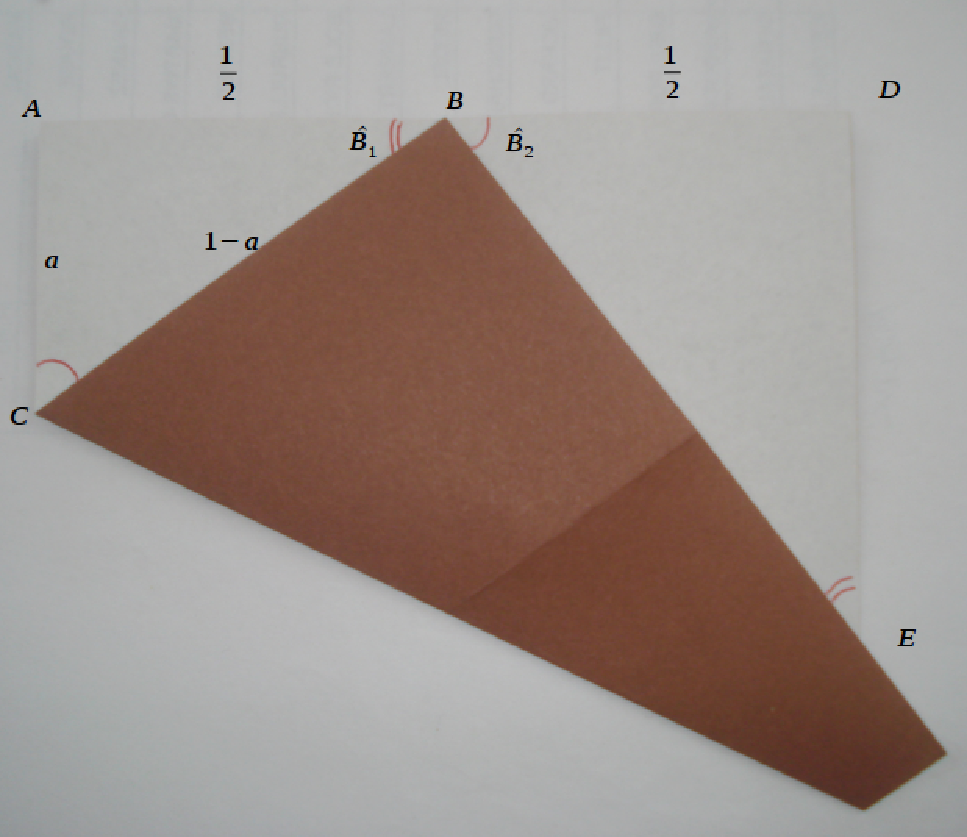
\includegraphics[width=5cm]{haga_coupe_anote}
    \end{center}


    Pythagore dans le triangle \( ABC\) : \( a^2+\left( \frac{ 1 }{2} \right)^2=(1-a)^2\).

    \( \Rightarrow \, a=\frac{ 3 }{ 8 }\).
    \end{multicols}

    
\newpage
\subsection{Théorème de Haga (angles)}
    \begin{multicols}{2}

    \begin{center}        
        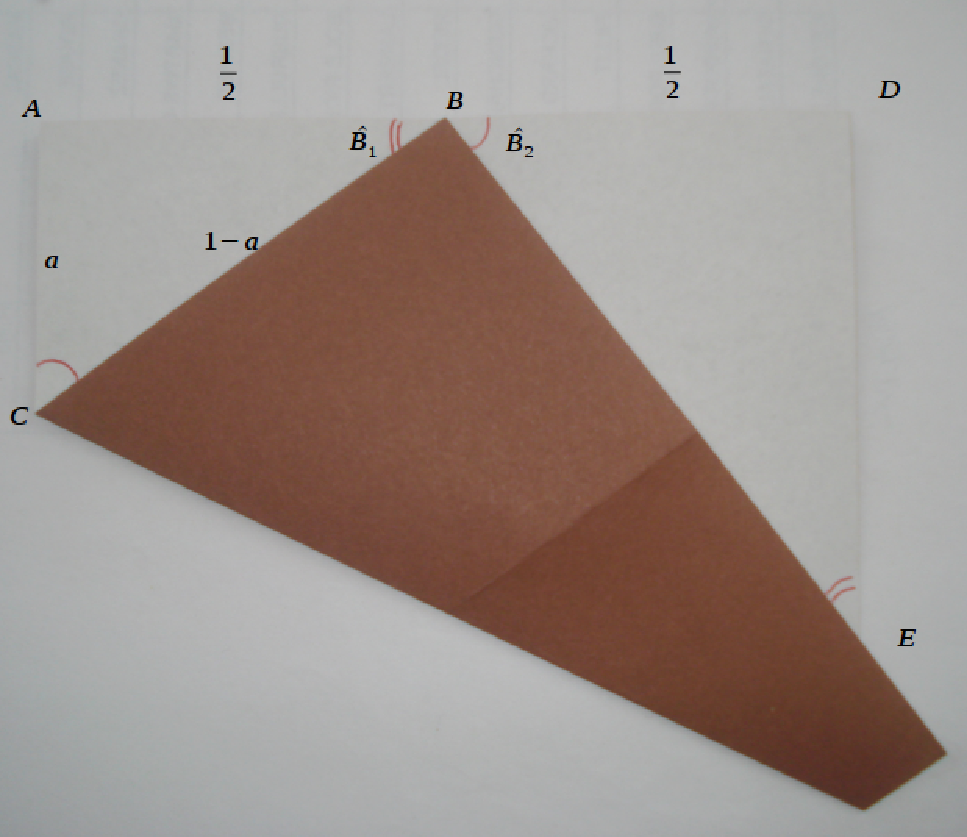
\includegraphics[width=5cm]{haga_coupe_anote}
    \end{center}

    \begin{subequations}
        \begin{numcases}{}
            \hat B_1+\hat B_2=90\\
            \hat B_1+\hat C=90\\
            \hat B_2+\hat E=90
        \end{numcases}
    \end{subequations}

    \( \Rightarrow \,   \hat B_2=\hat C \) et \( \hat B_1=\hat E\).
    \end{multicols}


    \begin{center}
        Les triangles \( ABC\) et \( BDE\) sont semblables.
    \end{center}

\newpage
\subsection{Théorème de Haga (proportionnalité)}
    \begin{multicols}{2}

    \begin{center}        
        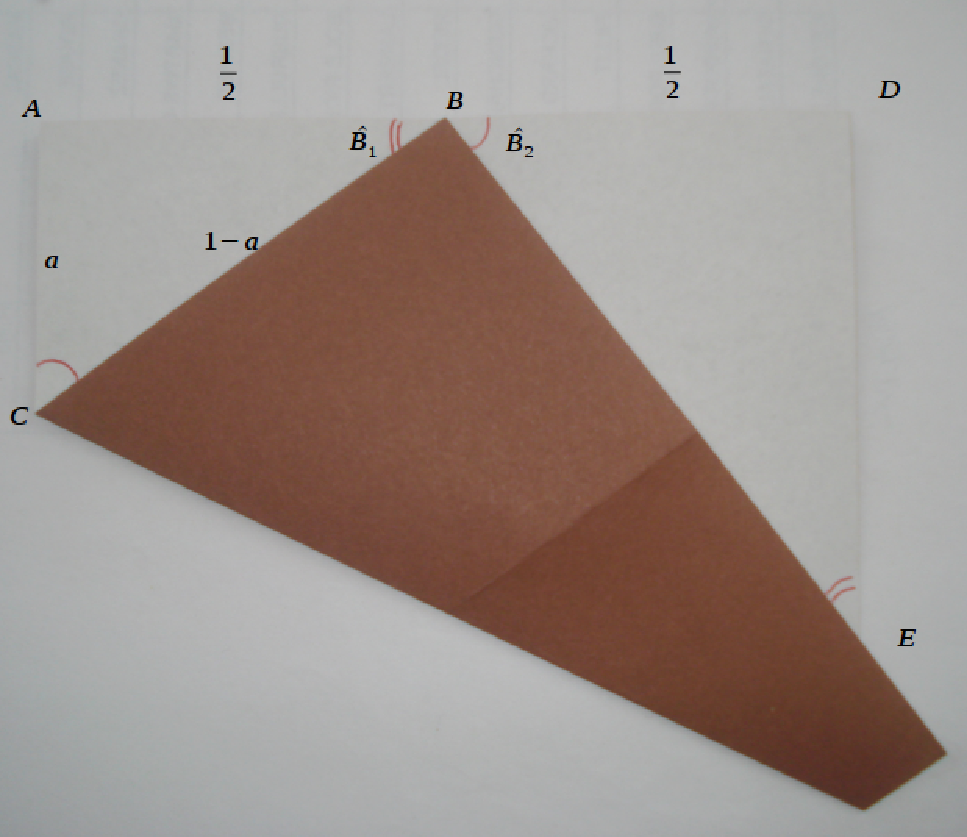
\includegraphics[width=5cm]{haga_coupe_anote}
    \end{center}

    \begin{equation}
        \frac{ DE }{ AB }=\frac{ BD }{ AC }
    \end{equation}
    \begin{equation}
        \frac{ DE }{ \frac{ 1 }{2} }=\frac{ \frac{ 1 }{2} }{ \frac{ 3 }{ 8 } }
    \end{equation}
    \begin{equation}
        2DE=\frac{ 4 }{ 3 }
    \end{equation}
    \begin{equation}
        DE=\frac{2}{ 3 }.
    \end{equation}
    \end{multicols}
